\documentclass[11pt,letterpaper,oneside]{article}
\usepackage[T1]{fontenc}
\usepackage[utf8]{inputenc}
\usepackage[margin=1in,headheight=15pt,footskip=30pt]{geometry}
\usepackage{newpxtext,newpxmath}
\usepackage[scaled=0.92]{sourcesanspro}
\usepackage[scaled=0.87]{inconsolata}
\usepackage{microtype,graphicx,xcolor,booktabs,tabularx,longtable,array}
\usepackage{amsmath,enumitem,listings,fancyhdr,titlesec,caption,needspace,float}
\usepackage[most]{tcolorbox}
\usepackage{tikz}
\usetikzlibrary{arrows.meta,positioning,calc}
\usepackage{hyperref}
\usepackage{bookmark}
\definecolor{ink}{HTML}{173247}
\definecolor{teal}{HTML}{087F8C}
\definecolor{muted}{HTML}{536370}
\definecolor{paper}{HTML}{F3F6F7}
\definecolor{add}{HTML}{14613C}
\definecolor{del}{HTML}{A02D37}
\hypersetup{colorlinks=true,linkcolor=ink,citecolor=teal,urlcolor=teal,
 pdftitle={Enabling HE Wi-Fi in FreeBSD},pdfauthor={Denis Lemire},
 pdfsubject={Architecture, implementation and validation of an experimental HE station path}}
\urlstyle{same}
\setlength{\parindent}{0pt}
\setlength{\parskip}{6.5pt plus 1pt}
\linespread{1.06}
\setlength{\emergencystretch}{2em}
\setcounter{tocdepth}{1}
\setcounter{secnumdepth}{2}
\titleformat{\section}{\sffamily\Large\bfseries\color{ink}}{\thesection}{0.7em}{}
\titleformat{\subsection}{\sffamily\large\bfseries\color{ink}}{\thesubsection}{0.7em}{}
\titleformat{\subsubsection}{\sffamily\normalsize\bfseries\color{teal}}{}{0em}{}
\titlespacing*{\section}{0pt}{20pt}{8pt}
\titlespacing*{\subsection}{0pt}{13pt}{5pt}
\captionsetup{font=small,labelfont={bf,sf},labelsep=period}
\pagestyle{fancy}
\fancyhf{}
\fancyhead[L]{\sffamily\small\color{muted}FREEBSD HE STATION SUPPORT}
\fancyhead[R]{\sffamily\small\color{muted}Denis Lemire}
\fancyfoot[L]{\sffamily\scriptsize\color{muted}Technical review draft\enspace /\enspace 5 November 2026\enspace /\enspace v0.2}
\fancyfoot[R]{\sffamily\small\thepage}
\renewcommand{\headrulewidth}{0.3pt}
\setlist{nosep,leftmargin=1.6em,topsep=5pt}
\newcolumntype{Y}{>{\raggedright\arraybackslash}X}
\newcommand{\code}[1]{\texttt{\small #1}}
\newcommand{\source}[1]{\textcolor{muted}{\small Evidence: #1.}}
\newcommand{\partpage}[2]{\Needspace{8\baselineskip}\section{#1}\label{#2}}
\newtcolorbox{finding}[1]{enhanced,breakable,colback=paper,colframe=teal,
 boxrule=0pt,borderline west={2pt}{0pt}{teal},arc=0pt,
 left=10pt,right=10pt,top=7pt,bottom=7pt,
 title={#1},coltitle=ink,colbacktitle=paper,fonttitle=\sffamily\bfseries}
\lstdefinestyle{base}{basicstyle=\ttfamily\footnotesize,backgroundcolor=\color{paper},
 frame=single,framerule=0pt,rulecolor=\color{paper},framesep=8pt,
 xleftmargin=8pt,xrightmargin=8pt,breaklines=true,breakatwhitespace=false,
 columns=fullflexible,keepspaces=true,showstringspaces=false,tabsize=4,
 captionpos=b,aboveskip=12pt,belowskip=8pt,
 keywordstyle=\bfseries\color{ink},commentstyle=\color{muted},
 stringstyle=\color{teal},numbers=left,numberstyle=\tiny\color{muted},numbersep=12pt}
\lstset{style=base}
\clubpenalty=10000
\widowpenalty=10000
\lstdefinelanguage{diff}{morecomment=[f][\color{add}]{+},
 morecomment=[f][\color{del}]{-},morecomment=[f][\color{teal}]{@}}
\begin{document}
\hypersetup{pageanchor=false}
\begin{titlepage}
\thispagestyle{empty}
\vspace*{0.45in}
{\sffamily\small\bfseries\color{teal}SYSTEMS ENGINEERING / TECHNICAL REVIEW\par}
\vspace{0.45in}
{\fontsize{37}{42}\selectfont\bfseries\color{ink}Enabling HE Wi-Fi\\in FreeBSD\par}
\vspace{0.3in}
{\sffamily\Large\color{muted}Architecture, implementation, debugging\\and experimental validation\par}
\vspace{0.5in}
{\Large Denis Lemire\par}
{\sffamily Aspiring independent contributor and FreeBSD enthusiast\par}
\vfill

\begin{tikzpicture}[x=1cm,y=1cm]
\draw[teal,line width=1.5pt] (0,0)--(15,0);
\foreach \x/\t/\b in {0/NEGOTIATE/Owned native state,5/OBSERVE/Actual driver behavior,10/VERIFY/Bounded reproducible tests}{
\node[anchor=north west,font=\sffamily\bfseries\small,text=ink] at (\x,-0.25) {\t};
\node[anchor=north west,font=\sffamily\small,text=muted] at (\x,-0.8) {\b};}
\end{tikzpicture}\par
\vspace{0.7in}
{\sffamily\small\color{muted}AUTHOR REVIEW DRAFT / v0.2 / 5 November 2026\par}
{\small A reviewer-oriented account of experimental 802.11ax station support,\\with explicit source identities, test boundaries and unresolved integration work.\par}
\vspace{0.2in}
{\footnotesize Not a FreeBSD Project publication or an assertion of upstream acceptance.\par}
\end{titlepage}
\pagenumbering{roman}\hypersetup{pageanchor=true}
\section*{Abstract}\addcontentsline{toc}{section}{Abstract}
This report describes an experimental native high-efficiency (HE, IEEE 802.11ax) station path in FreeBSD, connected through LinuxKPI to an existing rtw89 device driver. The work began with two independently scoped defects: a missing-station aggregation cleanup panic and a strong-signal RSSI narrowing error. Fixing the latter made a nearby Wi-Fi 6 access point usable in VHT mode and exposed a larger architectural gap between existing HE wire definitions, native association state, LinuxKPI peer records and driver consumers.

The implementation adds bounded native parsing and encoding, owned peer state, local-capability discovery, an opt-in association transaction, accepted-state mapping, rate calculation and receive metadata. Hardware testing subsequently exposed key-renewal ordering and lifetime problems and a separate aggregation-stop lock-contract panic. The report follows those failures through typed tracing and a matching kernel dump rather than attributing every symptom to HE.

Actual HE association and addressed receive traffic have been observed on the tested CURRENT and STABLE ports. Bounded wired traffic, renewal and integrity workloads pass for identified builds. The refreshed CURRENT review source now passes default-off VHT, HE software-crypto and HE hardware-crypto IPv6 controls, with WITNESS active and independently audited archives. Native STABLE control/reporting, IPv6 renewals and automatic HE startup also pass, including an ordinary default reboot followed by read-only data/integrity checks. These results do not establish general hardware compatibility, all optional HE functionality, suspend reliability or upstream acceptance.

\textbf{Scope:} one RTL8852BT station and one U6 Mesh access point, principally 5 GHz at 40 MHz. The initial design restricts station operation to at most 80 MHz. It does not claim AP mode, mesh mode, 6 GHz, 160 MHz, EHT or every optional HE mechanism.
\clearpage
\section*{How to use this report}\addcontentsline{toc}{section}{How to use this report}
I prepared this guide to make the design and its evidence inspectable. It is a technical draft under my name and subject to my review. Code, tests and this prose were developed with AI assistance; I remain responsible for checking their provenance and claims. No maintainer endorsement is implied.

Review the architecture and invariants first, then the implementation boundaries and validation matrix. The experiments distinguish a successful compile, a modeled path, an observed hardware path and a completed reliability workload. Each answers a different question. A passing collector is not by itself a passing workload, and an unexercised failure branch is not verified by the absence of another panic.

This edition records the November 5 Edmonton laboratory day, including results completed after midnight UTC on November 6. The signed CURRENT review branch is public at head \code{247377f}; all three refreshed-source controls and the separately identified STABLE startup/reboot checks have completed. Private raw captures and memory dumps remain excluded. Source identities and evidence classes are explicit: a helper model, firmware-fed cached rate, new firmware event and actual packet encoding are different observations. Unfinished review and coverage work is listed without an aggregate completion percentage.
\clearpage
{\small\setlength{\parskip}{0pt}\tableofcontents}
\clearpage\pagenumbering{arabic}
\section{Problem statement and tested system}
The concrete objective is a usable HE station implementation that fits FreeBSD's native networking architecture and can be reviewed for integration into CURRENT, with a separately identified STABLE port. Existing driver support for HE does not by itself supply native discovery, association, ownership and reporting semantics.

\begin{table}[H]\small\centering
\begin{tabularx}{\linewidth}{lY}\toprule
Component & Identified test configuration\\\midrule
Laptop & HP 15-fd0118ca; Intel N150; 4 GB RAM\\
Wireless & Realtek RTL8852BT; PCI 10ec:b520; subsystem 103c:88e9\\
Firmware & Version 0.29.122.1, build identifier 2ac94d05\\
Access point & Ubiquiti U6 Mesh; 5 GHz, channel 48, 40 MHz\\
Earlier CURRENT base & \code{7806832f23fb31d28386d42692b221776c9f4ee4}\\
Refreshed CURRENT base & \code{12f90bbd3029fedea93e9bb0b1f02c3afafe237b}\\
Published review head & \code{247377f1b50386c87d95fc53ed315d99e57ddf17}\\
STABLE base & \code{06e5b0422f3abf525472f6eb69677d7a32f4748f}\\
Compiler & FreeBSD Clang 21.1.8; separately built kernel object trees\\
Diagnostics & CURRENT WITNESS and INVARIANTS; STABLE GENERIC without them\\
Performance peer & Wired gigabit LAN peer running iperf 3.22\\\bottomrule
\end{tabularx}\caption{Hardware and source scope. RF conditions are a shared home environment.}\end{table}
The source identities are baselines with local experimental changes, not unmodified releases. The final public series explicitly includes the independently submitted missing-station guard and RSSI correction before the HE implementation. The older private HE-only sequence did not contain every runtime dependency; that distinction is now resolved in the end-to-end branch. Kernel, separate symbols, radio module, source changes and immutable experiment inputs are preserved together. A checksum establishes identity, not correctness.

\section{Architecture: where the handoffs were incomplete}
\begin{figure}[H]\centering
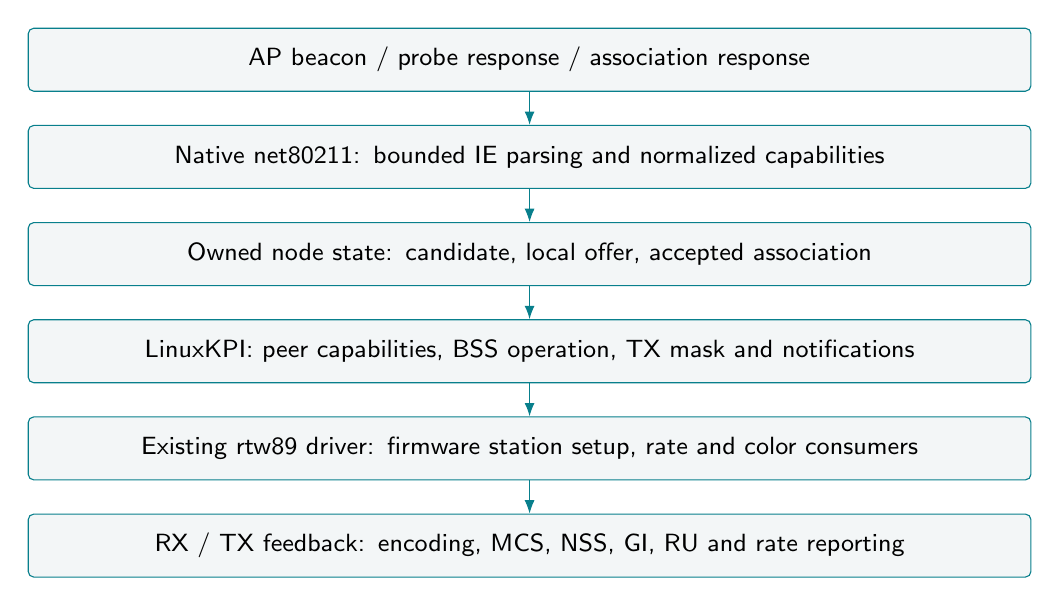
\begin{tikzpicture}[node distance=0.42cm,box/.style={draw=teal,fill=paper,rounded corners=2pt,text width=12.5cm,align=center,minimum height=0.8cm,font=\sffamily\small},arr/.style={-{Latex},color=teal}]
\node[box](wire){AP beacon / probe response / association response};
\node[box,below=of wire](parse){Native net80211: bounded IE parsing and normalized capabilities};
\node[box,below=of parse](state){Owned node state: candidate, local offer, accepted association};
\node[box,below=of state](kpi){LinuxKPI: peer capabilities, BSS operation, TX mask and notifications};
\node[box,below=of kpi](driver){Existing rtw89 driver: firmware station setup, rate and color consumers};
\node[box,below=of driver](rx){RX / TX feedback: encoding, MCS, NSS, GI, RU and rate reporting};
\draw[arr](wire)--(parse);\draw[arr](parse)--(state);\draw[arr](state)--(kpi);\draw[arr](kpi)--(driver);\draw[arr](driver)--(rx);
\end{tikzpicture}\caption{The HE station path spans native protocol state and an existing driver compatibility boundary.}\end{figure}
\subsection{Existing foundations}
The audited tree already contained native HE wire definitions and driver-facing HE records. The rtw89 driver already constructed local HE capabilities and consumed station/BSS HE information when setting up firmware. These are important foundations, and the implementation builds on them. It is not a replacement of rtw89 or a new radio driver.

The missing end-to-end connection was visible in source consumers: HT and VHT had native scan/association handoffs and LinuxKPI synchronization, while equivalent accepted HE peer state was not populated through the complete native station transaction. A decoder printing an HE element is diagnostic support; it does not show that the station offered, negotiated and used HE.

\subsection{Separation of meanings}
Four meanings must remain distinct: the AP's advertised capabilities, the radio's local capabilities, the station's transmitted offer, and the accepted association. Scan data can prepare a candidate, but cannot grant that candidate the privileges of an agreed link. Similarly, a configured HE switch does not prove negotiated HE, and negotiated HE does not prove the encoding of a particular data frame.

\section{Native parsing and capability intersection}
HE capability elements have variable layout. Optional 160 MHz and 80+80 MHz MCS/NSS maps affect the wire length, and PPE thresholds add variable bit fields. Copying the wire payload directly into a fixed in-memory structure would confuse compact optional slots and can overrun truncated input.

The parser checks the element identity, declared length, extension identity, fixed fields and each optional segment before copying. Missing optional maps normalize to unsupported. On failure, output is cleared so stale capabilities cannot survive a malformed update. The encoder performs corresponding length accounting before writing probe or association data.

Tests include all optional-bandwidth combinations, distinct map values to expose slot-order and byte-order mistakes, exact-length truncation, shortened declared lengths, PPE header combinations, malformed and duplicate elements, and a sanitized real AP capability fixture. The AP fixture's four-stream capability map is not treated as a four-stream local link: the actual adapter has two streams.

\subsection{Directional MCS maps}
Local transmit support intersects peer receive support; local receive support intersects peer transmit support. Unsupported stream entries remain unsupported. The implemented candidate path limits bandwidth and stream count to what the local radio and policy allow. Merely copying the AP's map into the local offer would over-advertise hardware capability.

\section{Ownership, lifetime and association transaction}
Borrowed pointers into receive mbufs are unsuitable as long-lived driver peer state. The implementation copies normalized records into owned node state and exposes snapshots. The accepted record is bound to the relevant node and channel/association context.

The first compile-successful association version was revised before boot: freeing an HE record at association cleanup could race a driver reader. The corrected lifetime retains the allocation until final node release; ordinary cleanup clears payload and flags. A dedicated leaf mutex protects writes and snapshot copies, with no other lock acquired while it is held. User-space tests model mutex operations as no-ops, so those tests cannot establish real kernel lock ordering.

\begin{figure}[H]\centering
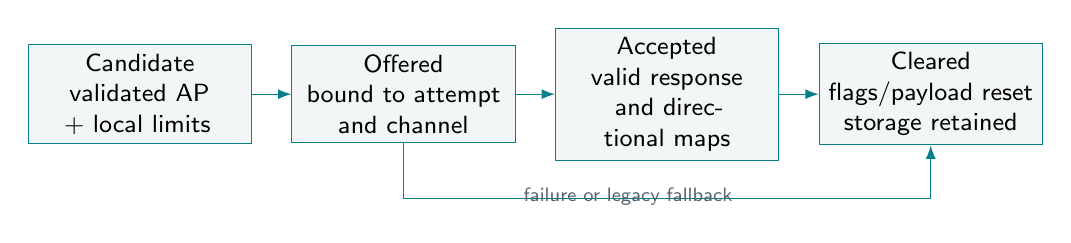
\begin{tikzpicture}[node distance=0.5cm,box/.style={draw=teal,fill=paper,text width=2.6cm,align=center,minimum height=1.1cm,font=\sffamily\small},arr/.style={-{Latex},color=teal}]
\node[box](c){Candidate\\validated AP + local limits};
\node[box,right=of c](o){Offered\\bound to attempt\\and channel};
\node[box,right=of o](a){Accepted\\valid response\\and directional maps};
\node[box,right=of a](x){Cleared\\flags/payload reset\\storage retained};
\draw[arr](c)--(o);\draw[arr](o)--(a);\draw[arr](a)--(x);
\draw[arr](o.south)--++(0,-0.7)-|(x.south);
\node[font=\sffamily\scriptsize,text=muted] at (6.2,-1.3) {failure or legacy fallback};
\end{tikzpicture}\caption{Logical association states. A candidate or configured switch cannot stand in for accepted peer state. Final node release, beyond this diagram, frees the allocation.}\end{figure}

\subsection{Acceptance conditions}
The station stages a local offer for a specific association attempt. An accepted HE response requires the corresponding offer, matching frequency, required QoS/HT/VHT state, valid capability and Operation elements, and compatible basic MCS requirements. Unsolicited, duplicate or malformed HE response data cannot create an accepted HE link. A valid legacy response without HE leaves HE disabled. Transmit error, teardown and reassociation paths clear stale offer or accepted state as appropriate.

The driver receives a snapshot of accepted state before its association consumer runs. Associated beacon Operation updates may update the existing peer after validation; scan allocation must not overwrite the current BSS's accepted state.

\section{LinuxKPI and driver integration}
LinuxKPI maps accepted native capabilities into the station's HE capability record and maps accepted operation/color state into BSS configuration. It supplies the expected change notifications and fills HE transmit masks from the peer's receive support. Zero-initialized HE transmit masks were a separate handoff gap: setting an HE boolean alone would not provide a usable rate policy.

The registration experiment separates HE from EHT. An independent HE registration gate defaults off; the existing EHT path continues to imply HE where required. The experiment identifies actual STA HE support and two-stream MCS 0--11 capability without claiming EHT support. This is a registration policy proposal requiring upstream review, not evidence that enabling EHT caused every earlier failure.

\subsection{Rate and receive metadata}
An original BSD implementation extends bitrate calculation for the HE inputs consumed by the driver, including bandwidth or RU allocation, guard interval and DCM. Boundary tests cover invalid combinations and rounding. The receive path preserves HE encoding, GI/RU/DCM semantics into native metadata. Layout checks on the tested amd64 builds preserve existing offsets and the 112-byte receive record; this is not an all-architecture ABI certification.

In the matched HE cohort, firmware rate-adaptation feedback included HE MCS 11, two streams and the 40 MHz width; the calculation consumer reported 5,735 units of 100 kbit/s, or 573.5 Mbps. This is firmware feedback and calculated PHY rate, not an external on-air capture or TCP capacity. The observed TCP medians are lower and measure a different quantity.

The userland display is tested on both CURRENT and the native STABLE port: he/-he changes configuration, status displays configured HE, and list sta tags accepted HE state. Real private utilities set both modes while independent readback/probes verify state and restoration. The existing VHT channel label remains independent of accepted HE and per-frame encoding. The provisional API still needs maintainer review. For the laptop's usable STABLE setup, a per-interface startup hook invokes the private utility before WPA; the base system utility remains unchanged. Ordinary reboot and non-root accepted-state display have been verified.

\section{Independent defects found during the work}
\subsection{Missing station during aggregation cleanup}
The original cleanup panic involved a missing LinuxKPI station during a native ADD-BA stop callback. A narrow NULL guard was submitted separately as FreeBSD GitHub PR 2531. This is distinct from the later mutex assertion. An existing public submission is not evidence that the patch has been integrated.

\subsection{Strong-signal RSSI narrowing}
Typed probes observed valid approximately -25/-26 dBm signal becoming negative native RSSI after conversion and signed narrowing. Saturating the scaled value prevents wraparound. The nearby AP then became usable for VHT association. PR 2532 contains that independently scoped fix. The initial symptom was misleading signal reporting/selection, not proof that the radio physically received a weak signal.

\subsection{Received DELBA and common-lock ownership}
A later VHT control workload panicked in \code{lkpi\_ic\_addba\_stop} while unconditionally dropping the common mutex. The matched dump showed an RX taskqueue path through native DELBA handling and an unowned common lock. The pinned mutex implementation calls WITNESS before the primitive unlock, so the zero lock word was not explained by the failing operation having already released it. WITNESS uses the lock object's identity; a truncated name alone does not demonstrate a naming collision.

The candidate records entry ownership, drops the lock only when owned, runs the existing driver operation, then restores the original ownership before the native handoff. Both kernel builds pass. Runtime observers check entry/handoff ownership and completed driver return. Both entry classes now have CURRENT runtime coverage: a complete VHT IPv6 renewal/load cohort observed 14 unowned received-DELBA calls and four owned teardown calls, all completing the actual driver operation with status zero and preserving entry ownership. The observer saved receive-path caller stacks. The latest STABLE VHT cohort has also completed with correct lock handoffs; its paired HE validation is still running at this edition checkpoint. No introducing commit or causal blame on HE registration has been established.

\section{Key renewal: ordering and lifetime}
Successful association and short traffic runs did not establish renewal reliability. Repeated pairwise-key replacement exposed connectivity loss in hardware and software encryption experiments. An ownership correction alone was insufficient.

Typed tracing later observed a protected EAPOL packet prepared with one key generation and reaching the PCI descriptor path after replacement. A separate observation captured native software encryption preparation overlapping key mutation. These observations support ordering/lifetime work; they do not establish a practical security exploit or simultaneous mutation inside an AES operation.

\begin{figure}[H]\centering
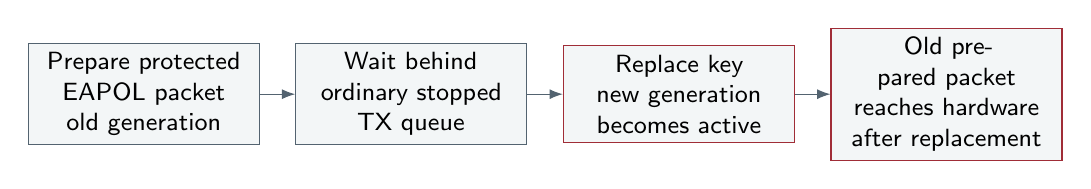
\begin{tikzpicture}[node distance=0.45cm,box/.style={draw=muted,fill=paper,text width=2.7cm,align=center,minimum height=1.1cm,font=\sffamily\small},arr/.style={-{Latex},color=muted}]
\node[box](p){Prepare protected\\EAPOL packet\\old generation};
\node[box,right=of p](q){Wait behind\\ordinary stopped\\TX queue};
\node[box,right=of q,draw=del](k){Replace key\\new generation\\becomes active};
\node[box,right=of k,draw=del](h){Old prepared packet\\reaches hardware\\after replacement};
\draw[arr](p)--(q);\draw[arr](q)--(k);\draw[arr](k)--(h);
\end{tikzpicture}\caption{Observed pre-fix ordering, shown as a sequence rather than a time-scale drawing. Control-port ordering and prepared-packet lifetime are separate review obligations.}\end{figure}

\subsection{Experimental corrections}
Native TX preparation is serialized under the relevant wireless lock. Key-update bracketing drains earlier native work and applies to software encryption too. EAPOL control-port traffic uses the existing direct transmit operation instead of waiting behind stopped TX queues. Prepared ordinary TXQ packets retaining an old key pointer are discarded before the old key is disabled, with completion after queue locks are released and the caller's node reference retained.

These are review-sensitive interfaces. The global taskqueue barrier and its self-member exception need lifecycle and lock-scope review beyond a successful workload. The ordinary-queue discard helper does not define the contract for packets already owned by the driver. Source inspection did not find an active remain-on-channel invocation in the audited LinuxKPI common source, but that bounded search is not proof of universal off-channel safety.

\begin{finding}{Coverage distinction}
The actual discard helper was tested with 4,101 modeled circular-queue cases, including positive removals and preservation of unrelated packets. Hardware traces observed helper calls but zero matching packet removals. The positive-removal branch therefore has modeled coverage, not demonstrated positive runtime coverage.\end{finding}

\section{Validation method and recovery}
Every disruptive trial uses immutable script copies, live observer readiness markers, an independent reconnect guard and a timed HE-off rollback. The permanent reboot default remains a known working environment. A detached evidence runner records command exit and a later complete barrier after final snapshots. The export waits for every worker's complete barrier, then checks workload, observer, guard and rollback status together.

The recovery design is deliberately bounded. A frozen kernel cannot execute a shell recovery script; matching binaries and symbols are preserved before boot, and normal reboot must retain a safe default. A configured hook is not counted as verified until its actual startup invocation has been observed. A temporary sleep inhibitor is verified after each boot; this prevents accidental sleep during tests and does not fix suspend/resume.

Diagnostics must also be bounded. One retry completed traffic but exceeded its trial deadline while nonnumeric netstat waited for name resolution. Numeric netstat completed in under 0.01 seconds while the nonnumeric command exceeded eight seconds. The retry now uses five-second-bounded numeric statistics and adequate outer deadlines. The earlier timed-out cohort remains failed.

\section{Evidence matrix}
\begin{longtable}{p{0.27\linewidth}p{0.36\linewidth}p{0.27\linewidth}}
\toprule Check & Observed result & Boundary\\\midrule\endhead
Native parser and ownership & Targeted normal and sanitizer suites; malformed/truncated/real IE fixtures & User-space execution is not kernel scheduling\\
Parser/IE fuzzing & 55,332,792 inputs, no sanitizer finding in recorded campaign & Not exhaustive protocol proof\\
HE arithmetic & 57,529 targeted checks & Does not measure on-air throughput\\
Receive metadata & 98,304 checks, preserved tested layout & Tested amd64 identities only\\
Association transaction & Allocation failure, unsolicited response, cleanup/reuse and fallback modeled & Mutex model does not validate ordering\\
CURRENT and STABLE builds & Separately built experimental kernels & Revisions and local diff matter\\
Actual HE association & Native acceptance, driver peer/BSS fields and addressed HE receive frames & One radio/AP setup\\
Wired renewal traffic & Completed bounded cohorts on both ports; integrity matches, no guard assistance & Different instrumentation/cohorts are not a causal comparison\\
Queued-key removal & Actual helper modeled, positive removals tested & No positive matching hardware discard yet\\
DELBA correction & CURRENT and STABLE positive received-DELBA and owned teardown coverage & Bounded observed paths, not all lifetime contracts\\
IPv6 & Both ports pass data/integrity, actual renewals and restoration; STABLE normal reboot passes & One AP/radio; earlier timer-only coverage gap retained\\
Suspend/resume & Prior hang unresolved & Inhibitor is a test control only\\
\bottomrule\end{longtable}

\section{Performance interpretation}
The wired endpoint removes the second wireless hop present in early Mac-hosted tests. A diagnostic CURRENT cohort measured four single-direction uplink/downlink samples with medians of 315.527 and 186.174 Mbps. It used per-packet tracing and cannot be presented as an uninstrumented capacity ceiling. Two later simultaneous bidirectional load intervals completed across renewals on each branch; these share airtime and are not equivalent to isolated one-direction samples.

\begin{table}[H]\small\centering
\begin{tabularx}{\linewidth}{lYY}\toprule
Cohort & Uplink / downlink (Mbps) & Interpretation\\\midrule
CURRENT diagnostic, sequential & Median 315.527 / 186.174 & Four samples, wired peer, per-packet observer\\
CURRENT simultaneous interval 1 & 143.112 / 128.757 & Two directions contend concurrently\\
CURRENT simultaneous interval 2 & 177.748 / 110.179 & Same bounded renewal cohort\\
STABLE simultaneous interval 1 & 203.420 / 97.805 & No WITNESS or INVARIANTS\\
STABLE simultaneous interval 2 & 191.994 / 103.974 & Same bounded renewal cohort\\\bottomrule
\end{tabularx}\caption{Earlier complete cohorts. These rows do not isolate a branch effect or an HE-versus-VHT speedup.}\end{table}
A fresh fixed-order VHT then HE comparison uses identical light instrumentation, kernel, module, AP and width. Its input manifest prevents staging edits between blocks. Both blocks completed with all workers passing, no guard reassociation request and no timed rollback assistance. Four samples per direction produced medians of 285.577/141.243 Mbps for VHT and 324.172/185.100 Mbps for HE. All eight integrity downloads matched. Both archives were independently copied and verified. The observed median differences are about 13.5 percent uplink and 31.1 percent downlink; this fixed-order comparison in shared RF is not a randomized estimate or a general AX performance claim. The rare stop-lock observer saw four owned handoffs in each block and no ownership mismatch, but no unowned handoff.

\section{IPv6 acceptance and observed renewals}
IPv6 was found disabled on the laptop interface, with no configured router solicitation daemon. After the completed IPv4 comparison, normal per-interface router-advertisement acceptance produced link-local and global addresses, a default route and three successful numeric peer pings. Duplicate-address detection completed. The configuration and daemon are now enabled in the current experimental environment. Both complete VHT/HE IPv6 data cohorts passed two sustained simultaneous TCP intervals, two integrity downloads and post-cleanup IPv6 peer checks, with no recovery intervention. An additional forced-IPv6 HTTPS fetch succeeded. The semantic key audit found three timed pairwise replacements in the VHT block and none in the HE block, despite read-back timer configuration of 60 seconds. Initial/cleanup key operations do not count as timed renewal. The HE data result remains valid, while HE renewal coverage remains unsatisfied for that cohort. The diagnostic repetition subsequently completed four renewal requests, four negotiations and four actual timed replacements, with complete workload/guard success. A sequential repeat removed the per-packet hardware probe and also completed four requests and four timed replacements with data/integrity and clean restoration. These runs establish positive renewal coverage without explaining the original missing-renewal observation. The original result and its limit remain in the record.

The latest STABLE pair completed both modes with all collectors passing and no recovery intervention. Actual timed replacements numbered three in VHT and four in HE; four requests were seen in each mode, so not every VHT request completed. The same real native utility set both modes and displayed accepted state. Received DELBA caller stacks accounted for six unowned VHT handoffs and two unowned HE handoffs, plus four owned teardown handoffs in each mode, with zero ownership mismatches or incomplete driver operations. IPv6 startup, data, integrity and restoration passed. Global addresses alone are not the acceptance criterion; private prefixes and addresses remain outside this report.

\section{Refreshed controls and automatic startup}
The final review branch builds on refreshed main with GENERIC, rtw89, iwlwifi, mt76, ZFS and matching tracing/auxiliary modules. Intel and MediaTek have compile coverage only. All 21 commits have verified Denis Lemire author/committer identity, DCO sign-off and cryptographic signatures; GitHub independently reports every signature valid. Final whitespace and FreeBSD style checks pass. The sixteen changed implementation files match the earlier tested source bytes; manual text differs. Fresh builds and runtime, rather than that byte comparison alone, establish the new-base checkpoint.

The final CURRENT kernel identity begins \code{f4652f8e63cd}; the radio module begins \code{888f950817b2}. Kernel and userland report 16.0-CURRENT, but the existing 16-series userland was not rebuilt for these 35 upstream commits. All three controls use the same binaries. The default-off boot leaves HE registration unset in loader layers and verifies its compiled zero default; EHT is zero. The two HE controls enable HE registration while selecting software or hardware crypto separately.

\begin{table}[H]\small\centering
\begin{tabularx}{\linewidth}{lYY}\toprule
Fresh CURRENT control & Measured sender up/down, Mbps & Acceptance scope\\\midrule
Default-off VHT & 279.393 / 134.419 & One-direction IPv6 samples; legacy mode and integrity\\
HE, software crypto & 39.068 / 17.328; 38.238 / 16.969 & Two simultaneous 120 s intervals; four completed renewals; zero driver key installs\\
HE, hardware crypto & 191.260 / 100.436; 185.904 / 103.547 & Two simultaneous 120 s intervals; four completed renewals; six pairwise installs including initial/cleanup\\\bottomrule
\end{tabularx}\caption{Fresh-source controls pass all collectors without recovery assistance. Different profiles are not direct speed comparisons.}\end{table}
The slower software-crypto path is retained as a limitation, not hidden behind the functional pass. Its cause has not been isolated. All five synthetic integrity downloads across these controls matched. Shared RF, short intervals and instrumentation limit performance interpretation; retransmissions remain in the machine-readable evidence.

\subsection{Making the tested laptop usable after reboot}
A separate STABLE clone uses the already tested kernel/module set and a private native utility. FreeBSD's per-interface startup hook runs after wlan creation and before WPA. It enables HE without replacing the base ifconfig. Effective HE/EHT/crypto settings, native accepted HE, both IP routes and exact artifacts verify after startup. Read-only IPv4/IPv6 traffic and integrity checks then pass without HE setters, WPA mutations or fallback assistance. The tested clone was selected as normal default, its temporary boot-return service disabled, and an ordinary reboot repeated those checks. The previous RSSI-fixed environment remains selectable.

One startup attempt deliberately remains incomplete: traffic/integrity and accepted HE passed, but a firmware-event observer attached after association emitted no new rate reports. Its deadline guard restored legacy mode. A later typed snapshot at the exported TX-dequeue boundary read the current station's firmware-fed rate cache: HE flags, MCS 11, two streams, 40 MHz and calculated 573.5 Mbps. Source shows this cache is populated by firmware reports and is also used by the driver's station-statistics callback. A legacy control produced VHT flags instead. This is current-station cached firmware evidence, not a new C2H event or the encoding of the particular sampled packet. No driver change was made to obtain it; the failed observer attempt is preserved.

The two complete startup/reboot cohorts each transferred data in both directions over IPv4 and IPv6 and verified both 8 MiB payload hashes. The ordinary-boot receiver samples were 280.725/192.343 Mbps for IPv4 and 271.710/133.526 Mbps for IPv6. These are single samples in shared RF, not family-performance conclusions. HE remains enabled after acceptance. Suspend/resume and broad hardware reliability are still unverified.

\section{Review boundaries and integration path}
The public feature should be an end-to-end testable branch composed of logical commits: native parser/encoder, owned peer lifecycle, hardware capability handoff, association transaction, LinuxKPI mapping, bitrate, receive metadata/reporting and explicit driver enablement. Independently useful defect fixes remain separate. Preserve the original signed experimental history before reorganizing it into a review series.

CURRENT is the upstream target. The published end-to-end branch is \url{https://github.com/denislemire/freebsd-src/tree/codex/80211ax-sta-review}, based on \code{12f90bbd3029}. It contains 21 signed logical commits across 17 files, with 1,313 insertions and 46 deletions. The original signed experimental history is preserved separately. The standalone helper kit records source/compiler/input identities; its extracted archive itself passed normal and ASan/UBSan suites. STABLE results document a separate port, not an integrated backport.

The intended first contact is one factual freebsd-wireless email, with Bjoern Zeeb, Adrian Chadd and Colin Percival copied, linking code, this guide and reproducible tests. Pinned MAINTAINERS requests wireless-list pre-commit review for net80211 and the LinuxKPI Phabricator group for that component. The email remains an author-review draft; no feature PR, mailing-list message or formal review request has been sent. One canonical review trail should follow maintainer guidance. A substantial native protocol feature need not use the same route as the two small independent bug-fix PRs.

\subsection{Licensing and provenance}
New native implementation and experimental tooling use BSD licensing and existing FreeBSD wire definitions. Existing contributed driver licenses and attribution must be preserved. GPL-only implementation must not be copied into BSD native files, including through translation. The touched rtw89 core file explicitly carries \code{GPL-2.0 OR BSD-3-Clause} and Realtek attribution; it is dual licensed, not GPL-only. Native HE retains its BSD-2-Clause notices, and LinuxKPI retains its existing two-condition BSD notice. The final 17-file header/notice audit preserves those licenses and the existing BSD-3-Clause ifconfig/manual notices. Model output is not a substitute for inspecting that inventory.

\section{Remaining review and coverage work}
\begin{enumerate}
\item Obtain architectural/component review of capability policy, native peer and operation ownership, the provisional control API, reporting semantics and cross-driver key/queue contracts.
\item Extend hardware/AP and longer-soak coverage. The tested AP width is 40 MHz; 80 MHz hardware operation, GTK lifecycle, extensive roaming, firmware recovery and suspend/resume remain unverified.
\item Investigate the slower software-crypto path separately. Preserve the working hardware-crypto results and distinguish positive modeled queue removal from the still-unobserved live positive discard branch.
\item Agree on integration of the standalone helper suites into the project's test framework, and broaden meaningful architecture/build coverage beyond tested amd64 identities.
\item Follow review through CURRENT integration, then any committer-approved, separately validated stable/15 backport. No acceptance or integration date is promised.
\end{enumerate}
The completed controls establish a bounded, reproducible experimental station implementation on this laptop. They do not certify every optional Wi-Fi 6 feature or all FreeBSD wireless hardware.

\clearpage
\appendix
\section{Terminology for reading traces}
\begin{longtable}{p{0.19\linewidth}p{0.73\linewidth}}\toprule Term & Meaning in this report\\\midrule\endhead
HT / VHT / HE & High Throughput (802.11n), Very High Throughput (802.11ac), High Efficiency (802.11ax). Capability, channel configuration and actual frame encoding are separate evidence.\\
VHT/40 & A VHT-labelled channel configured for 40 MHz; not proof that no HE frames are used.\\
MCS & Modulation and coding index; interpreted with NSS, bandwidth/RU, GI and other parameters.\\
NSS & Spatial stream count. A four-stream AP does not make a two-stream client four-stream.\\
GI & Guard interval between symbols; must match the encoding's defined values.\\
RU & Resource unit, a frequency allocation used by HE; not simply a channel width label.\\
DCM & Dual-carrier modulation; a rate-relevant capability/input with restricted combinations.\\
PPE & Packet padding threshold information; variable-length capability data requiring bounds checks.\\
BSS color & HE BSS identification information; validated operation state is required before driver use.\\
AMPDU / BA & Aggregated MAC protocol data units and Block Ack agreement. DELBA terminates an agreement.\\
EAPOL / PTK & Authentication/key-management protocol traffic and pairwise transient key; renewal tests must observe ordering through replacement.\\
WITNESS & FreeBSD lock diagnostics. A no-panic interval is not proof that every lock path ran.\\
INVARIANTS & Additional kernel consistency checks, enabled in the identified CURRENT configuration.\\
SLAAC / ND & IPv6 stateless address autoconfiguration and neighbor discovery; both require functional control traffic.\\\bottomrule\end{longtable}

\clearpage
\section{Reviewer map: source boundaries and invariants}
This appendix navigates the public experimental review head \code{247377f}. Symbol names are more useful than transient line numbers during review. The 17-file, 21-commit series includes both independent dependency fixes and the lock, registration and user-visible reporting changes. The complete branch, not an older private HE-only history, identifies the runtime source contract.

\begin{longtable}{p{0.31\linewidth}p{0.61\linewidth}}\toprule Boundary & Review focus\\\midrule\endhead
\path{sys/net80211/ieee80211_he.c} & Native capability/Operation parser, encoder, directional map intersection, candidate construction and owned association state. Check bounds, policy and failure clearing separately.\\
\path{sys/net80211/ieee80211_he.h} & Native API, maximum lengths and peer snapshot contract. Review ownership and caller preconditions.\\
\path{sys/net80211/ieee80211_node.c} & Node creation, cleanup and final release. Check that cleanup invalidates state without freeing storage still visible to readers.\\
\path{sys/net80211/ieee80211_input.c} & Beacon/probe parameter parsing. Check extension identity and available input length.\\
\path{sys/net80211/ieee80211_output.c} & Outgoing association element accounting, error rollback and recording of the transmitted offer.\\
\path{sys/net80211/ieee80211_sta.c} & Received association acceptance and later operation updates. Check legacy fallback and unsolicited state.\\
\path{sys/net80211/ieee80211_ioctl.c} & Provisional opt-in control. Review API allocation and policy with maintainers.\\
\path{sys/compat/linuxkpi/common/src/linux_80211.c} & Local capability callback, accepted peer/BSS mapping, rate masks, RX metadata, key/queue ordering and common-lock preservation. These need distinct review units.\\
\path{sys/contrib/dev/rtw89/core.c} & Separate HE/EHT registration gate; preserve existing driver license, attribution and unaffected build behavior.\\
\path{sbin/ifconfig/ifieee80211.c} & CURRENT and native STABLE control/status/station reporting are built and hardware tested. Final API review remains required.\\\bottomrule\end{longtable}

\subsection{Invariants to check at each interface}
\begin{enumerate}
\item Input parsing never reads past the received element extent, even if a declared length claims more bytes. Failure must clear output.
\item Stored peer state owns its bytes after the receive buffer is freed. A pointer into an mbuf is not an owned capability.
\item A scan candidate cannot set the accepted HE node flag. A locally enabled knob cannot substitute for a received accepted response.
\item The local offer belongs to the relevant attempt/channel and respects local hardware and native policy. A peer's stronger capabilities cannot inflate the local radio.
\item TX/RX MCS intersections use opposite local/peer directions and explicit endian conversions.
\item Driver-facing HE information is prepared before the driver consumes the association and cleared when that association ends.
\item Node cleanup invalidates negotiation; final node release owns deallocation. Snapshot copies must obey the actual kernel lock contract.
\item Callback exit restores entry common-lock ownership. An unlocked receive caller must remain unlocked; a locked teardown caller must receive its lock back.
\item An old key cannot be freed while prepared packets retain an unsafe reference. Native queue ownership and driver-owned descriptors require distinct contracts.
\item User-visible state states what was actually measured: configured, accepted, frame encoding or calculated rate.
\end{enumerate}
None of these invariants is established merely because the corresponding field name exists. Review both producers and consumers, including failure and cleanup paths.

\section{Reproducing the protocol tests}
The test strategy has several layers. Pure wire-layout routines run as ordinary user-space code against native definitions. Extracted actual-routine harnesses exercise code used by the implementation rather than a second independent approximation. Kernel builds validate compiled integration. Runtime probes then establish which paths the real hardware exercised.

\subsection{Wire parser and encoder experiments}
Start with a pinned source tree and a recorded compiler. Run the normal suite, then the address/undefined-behavior sanitizer variant using the same inputs and definitions. Repeat with the separately pinned STABLE definitions. Record exact command lines and return statuses, not only a final test-count banner.

For capability parsing, use distinct values in every optional MCS map. Include a case with the sparse optional combination that a fixed-structure copy would misinterpret. Pass buffers whose actual allocation ends exactly at each truncated length, so an over-read is visible to the sanitizer. Check cleared output after each failure, including a malformed input immediately after a successful parse.

The lab test package uses the following ordinary-user commands on FreeBSD, substituting an already pinned and patched source tree. These are test-package entry points, not commands that install a kernel:
\Needspace{13\baselineskip}
\begin{lstlisting}[caption={Native parser and pure-protocol suite entry points.}]
make NET80211_SYS=/path/to/pinned/src/sys native native-sanitize
make NET80211_SYS=/path/to/pinned/src/sys \
    ownership ownership-sanitize mcs mcs-sanitize \
    operation operation-sanitize peer peer-sanitize \
    encode encode-sanitize
\end{lstlisting}
The ownership and peer targets require their generated actual-routine headers from the matching source. Preserve the extraction scripts and generated header identities with the run. The final public test package still needs packaging beside the review branch.

For encoding, test output capacity one byte below required size, exact size and excess capacity. Verify the output length and the parsed round trip. A parser/encoder round trip alone can let paired bugs agree, so retain independent expected byte fixtures. The real AP fixture is sanitized to the HE element only, without neighboring network identifiers.

\subsection{Association and lifecycle harness}
Exercise an eligible candidate, absent local hardware support, disabled native HE, missing QoS/HT/VHT, unsupported channel width, allocation failure and transmit failure. A received response must be tested with and without an offer, on the original and changed channel, with malformed/duplicate elements and with a valid legacy fallback.

After acceptance, destroy or modify the original receive buffer and confirm the owned record still contains the accepted values. Then exercise cleanup, reuse, accepted Operation updates and final release. Check both directional maps with asymmetric local and peer support. Tests that replace kernel mutexes with no-ops validate state transitions and ownership of memory, not mutual exclusion or lock-order safety.

\subsection{Key-retirement queue model}
The extracted helper's circular-queue cases include empty queues, wraparound, every key match, no key match, mixed matching/unrelated packets and preserved order. Verify both the number removed and the identity/order of survivors. Completion must occur after queue locks are dropped. The recorded campaign exercised 111,767 removed and 111,205 preserved packets across 4,101 cases.

Run normal and sanitizer versions on the Mac and the two native FreeBSD definition sets. Then ask the different runtime question: did the hardware workload create a matching queued packet at retirement? In the recorded passing cohorts the answer is no. The model's positive-removal result must not be relabelled as a positive live removal.

\section{Reproducing a bounded hardware trial}
Use an experimental boot environment and preserve the normal reboot default. Before boot, copy the exact executable, separate symbols, loaded-driver candidate, source diff, kernel configuration and build/install logs into protected evidence storage. Verify checksums on an independent machine before overwriting a reproducer.

\subsection{Preflight checklist with a purpose}
\begin{enumerate}
\item Verify the running kernel hash, root boot environment and loaded module identities. Installed files and running images can differ after an incomplete boot/install cycle.
\item Confirm native HE is initially disabled and normal association completes. Record the actual accepted AP/channel without putting its identifying data into public results.
\item Verify a bounded sleep inhibitor is registered. Restart it after boot and release it at handoff.
\item Compile each typed DTrace program on the running kernel. A probe that cannot compile must not silently become a missing observer.
\item Start the observer, guard and timed rollback detached. Read live readiness markers before requesting association changes.
\item Execute immutable copies of the controller and worker. Keep hashes of inputs and reject a changed input set between comparison blocks.
\end{enumerate}
The controller pins the intended AP only in memory, requests a disconnect, applies the explicit HE setting and requests reassociation. It requires completed WPA and the intended peer, then checks network readiness. After the data workload it restores HE off, the original AP preference and any in-memory renewal interval. It does not save supplicant configuration.

\subsection{Why several completion records exist}
The measured command can exit before the collector has taken its final system snapshot. The command-exit file therefore is not the final barrier. Wait for each collector's completion record; only then read all statuses and archive. Check guard reassociation requests and timed rollback assistance independently. A successful transfer recovered by a guard is an assisted result, not an unassisted reliability pass.

The outer deadline covers startup, the longest child guard and final snapshots. FreeBSD timeout can terminate descendants even if they daemonize, so a deadline calculated from traffic duration alone is insufficient. Interrupted exports remain explicitly partial. Never create a missing completion marker to make an interrupted experiment look finished.

\subsection{When SSH disappears}
An SSH disconnect is an observation about the management connection, not a diagnosis of panic. Check a second independent endpoint, boot uptime and crash metadata. Let detached recovery continue. If a new panic dump exists, preserve it with the matching image before changing kernels. If the kernel is frozen, a shell rollback cannot run; human console recovery may be necessary. Keep these cases separate in the evidence.

\section{LLDB: from a panic to a lock-contract claim}
The DELBA panic illustrates the chain of evidence needed for a narrow kernel diagnosis. Opening a core without the matching executable can produce an apparently loaded target with unusable threads or types. Load the executable and separate symbols, then verify readable kernel globals and thread enumeration.

\Needspace{13\baselineskip}
\begin{lstlisting}[caption={Debugger setup pattern; substitute preserved matching artifacts.}]
lldb --core /protected/evidence/vmcore.N \
    /protected/evidence/kernel
(lldb) target symbols add /protected/evidence/kernel.debug
(lldb) target variable dumptid
(lldb) thread list
\end{lstlisting}
Derive the debugger's thread index from the crashed thread ID for that dump. The index is not the same identifier as the kernel thread ID. Select the derived index and inspect the complete stack before choosing a source frame.

\Needspace{13\baselineskip}
\begin{lstlisting}[caption={Typed inspection after selecting the actual crashed thread and callback frame.}]
(lldb) bt
(lldb) frame variable ni tap
(lldb) frame variable ni->ni_ic->ic_comlock
(lldb) frame variable -f hex ni->ni_flags
\end{lstlisting}
For the observed dump, the meaningful caller chain was receive taskqueue, native station input, LinuxKPI management receive, native BA DELBA handler, LinuxKPI ADD-BA stop, mutex unlock and WITNESS. The common mutex word was zero and the node's private HE bit was clear. This explains why the failure must not be described as an HE-only transmit failure.

\subsection{Interpret values using the compiled source}
Read the pinned mutex constants and implementation. In this source, zero is the unowned mutex state. Read the order of WITNESS and primitive unlock: the assertion runs before the unlock, which rules out the tempting explanation that the failing operation itself had already cleared the lock word. Read WITNESS's object-identity lookup before attributing the assertion to a truncated lock name.

A source tree can change after a matching executable and symbols have been preserved. Map the debugger's compiled source paths to immutable preserved source before relying on displayed lines. Matching symbols identify locations and types; they cannot make a mutable source file match the crashed build.

\subsection{Small correction, several caller contracts}
The callback has teardown, explicit AMPDU stop and received DELBA callers. Some hold the common mutex and others need not. The proposed correction preserves ownership around the existing driver operation:

\Needspace{13\baselineskip}
\begin{lstlisting}[language=C,caption={Candidate ownership preservation around an existing driver call.}]
icislocked = IEEE80211_IS_LOCKED(ic);
if (icislocked)
    IEEE80211_UNLOCK(ic);
wiphy_lock(hw->wiphy);
error = lkpi_80211_mo_ampdu_action(hw, vif, &params);
wiphy_unlock(hw->wiphy);
if (icislocked)
    IEEE80211_LOCK(ic);
\end{lstlisting}
This excerpt does not establish all node/station lifetime assumptions in the surrounding callback. It addresses the demonstrated unconditional-unlock assumption. Review the complete function and actual caller references, not only the changed lines.

\section{DTrace: observing semantics without overclaiming}
Typed probes are preferable to guessed offsets. First verify the running type/layout and probe availability. Read entry arguments at entry and return values at return; compiler optimization and tail calls can make a wrapper's return an unreliable point for inferring a later handoff.

The rare aggregation-stop observer saves the common-lock identity and whether the current thread owned it at callback entry. It observes the actual driver AMPDU call and its return, then compares ownership at entry to the native \code{ieee80211\_addba\_stop} handoff. This avoids assuming the wrapper's return corresponds to a non-tail-called operation.

The audit reports total handoffs, owned and unowned driver handoffs, ownership mismatches, incomplete driver operations and malformed records. Mismatch/incomplete/malformed are failures. Zero unowned observations is a coverage gap, even when every observed owned call succeeds. Caller stack aggregates help establish whether the receive path actually ran.

\subsection{Key and mode observations}
A key-generation label is local experiment metadata. It helps follow preparation, queueing, replacement and hardware handoff without printing key material. A descriptor observed after replacement can demonstrate an ordering crossing; an 802.11 ACK alone cannot establish that an EAPOL message was accepted at the protocol level. Likewise, a software AMPDU flag is not proof of actual on-air aggregation.

Mode evidence combines native acceptance, driver station/BSS state and addressed data encoding. Capabilities in an AP beacon, a successful ioctl or a configured HE switch are insufficient alone. Firmware-consumer evidence and rate metadata provide complementary checks, with their own interpretation limits.

\subsection{Instrumentation changes the experiment}
Per-packet probes add work at a sensitive path. They are valuable for a key-ordering diagnosis and unsuitable for claiming an uninstrumented throughput ceiling. The matched performance comparison therefore uses identical lighter observers in both modes. Keep diagnostic and performance cohorts separately named and never compare them as though only HE enablement changed.

\section{Artifact ledger and reproducibility boundaries}
The following digest identifiers refer to complete privately preserved evidence archives, not public download locations. Public packaging should provide a sanitized machine-readable ledger alongside the eventual review branch. Full memory, key-bearing state and identifying network captures stay protected.

\begingroup\renewcommand{\arraystretch}{1.05}
\begin{longtable}{p{0.29\linewidth}p{0.63\linewidth}}\toprule Artifact & SHA256 identity\\\midrule\endhead
Matched VHT IPv4 & {\scriptsize\texttt{0321fe057da01d3771919bb658c712ebd538cd05d958254d343d448849bca7f7}}\\
Matched HE IPv4 & {\scriptsize\texttt{39bac08742c6c186a51324329fac76325b235972b2b908c33afa7a7be6686fb6}}\\
DELBA matched dump set & {\scriptsize\texttt{6b563d432b3f68247c3508c9dae7c16f2d71112816ba16f81531ccc5f3cec2bb}}\\
CURRENT wired renewal & {\scriptsize\texttt{3fd3b588230b67edac43491a609b31b72d0e29161dd5240bb23568d6532213a1}}\\
CURRENT wired concurrent load & {\scriptsize\texttt{5c3b428d814ff957aec4ae3b711009c5e5dcb8d952c09570abb8c127326922fe}}\\
STABLE wired concurrent load & {\scriptsize\texttt{d781767dd81e1116af8f508776aef194d9a1a6010c08adc148aaaaa6ec108a2d}}\\Fresh CURRENT default-off & {\scriptsize\texttt{08020de42991b4e156603689d3aba6154826d7dbb06b30d89872b74b1fac2c10}}\\
Fresh CURRENT software crypto & {\scriptsize\texttt{a32b55200e0b0c0d3e747b0b01d20b9ff6703d8873ece6514213e737eb52a99c}}\\
Fresh CURRENT hardware crypto & {\scriptsize\texttt{0012b71f77ca3e283b35e5c0e4fe307f02f3f03a294f0979b1f6b134c51b8931}}\\
Native STABLE VHT IPv6 & {\scriptsize\texttt{4f25547666588e7a846e156d00317e8d42095fd5d033466a0967186690376fe8}}\\
Native STABLE HE IPv6 & {\scriptsize\texttt{57cb73cdab6ff12c6da19c6507fc2815db0eec8532bb389894f0c0bf80e35863}}\\
Automatic HE startup & {\scriptsize\texttt{f5ace853a02ff3b61b5db3c847f5d5cd2cf27db6c8b54054e0fce246f194b1dc}}\\
Ordinary default HE reboot & {\scriptsize\texttt{e6efd2f96cba3742c1a506dc64ce17a68e63106b1af64e8e91584a835b09a48a}}\\
\bottomrule\end{longtable}\endgroup
Preserve exact binaries/symbols, source and configuration, compiler/debugger versions, immutable scripts, raw results, collector completion, integrity hashes and recovery records for each cohort. Distinguish trial-time identities from fallback/export state. Verified independent copies protect evidence; they do not reproduce an experiment. External reproduction still requires accessible source, a defined workload and another hardware execution.

\clearpage
\section{Selected public sources}
\begin{enumerate}
\item Published signed review source: \url{https://github.com/denislemire/freebsd-src/tree/codex/80211ax-sta-review}.
\item Component review expectations: pinned FreeBSD \path{MAINTAINERS} at \code{12f90bbd3029}.
\item FreeBSD contribution guide: \url{https://docs.freebsd.org/en/articles/contributing/}.
\item FreeBSD native HE definition work: commit \code{2ab7cbdc346e}, review \url{https://reviews.freebsd.org/D50677}; related structure migration \url{https://reviews.freebsd.org/D50676}.
\item Foundation Wi-Fi 6 tracking: \url{https://github.com/FreeBSDFoundation/proj-laptop/issues/34}. An open tracking issue is not proof that no unpublished work exists.
\item Independent cleanup fix: \url{https://github.com/freebsd/freebsd-src/pull/2531}.
\item Independent RSSI fix: \url{https://github.com/freebsd/freebsd-src/pull/2532}.
\item FreeBSD Handbook IPv6 configuration: \url{https://docs.freebsd.org/en/books/handbook/network/}.
\end{enumerate}
\end{document}
